\documentclass{article}

% if you need to pass options to natbib, use, e.g.:
%     \PassOptionsToPackage{numbers, compress}{natbib}
% before loading neurips_2018

% ready for submission
% \usepackage{neurips_2018}

% to compile a preprint version, e.g., for submission to arXiv, add add the
% [preprint] option:
%     \usepackage[preprint]{neurips_2018}

% to compile a camera-ready version, add the [final] option, e.g.:
\usepackage[preprint]{neurips_2018}

% to avoid loading the natbib package, add option nonatbib:
%     \usepackage[nonatbib]{neurips_2018}

\usepackage[utf8]{inputenc} % allow utf-8 input
\usepackage[T1]{fontenc}    % use 8-bit T1 fonts
\usepackage{hyperref}       % hyperlinks
\usepackage{url}            % simple URL typesetting
\usepackage{booktabs}       % professional-quality tables
\usepackage{amsfonts}       % blackboard math symbols
\usepackage{microtype}      % microtypography
\usepackage{graphicx}
\usepackage{float}

% \usepackage{verbatim}
\usepackage{amsmath}
\usepackage{amssymb}
\usepackage{algorithm}
\usepackage{amsthm}
\usepackage{algorithmic}
\newtheorem{theorem}{Theorem}
\newtheorem{proposition}{Proposition}
\newtheorem{corollary}{Corollary}
\newtheorem{lemma}{Lemma}
\newtheorem{remark}{Remark}

\usepackage{xcolor}

\title{Bandit networks}

% The \author macro works with any number of authors. There are two commands
% used to separate the names and addresses of multiple authors: \And and \AND.
%
% Using \And between authors leaves it to LaTeX to determine where to break the
% lines. Using \AND forces a line break at that point. So, if LaTeX puts 3 of 4
% authors names on the first line, and the last on the second line, try using
% \AND instead of \And before the third author name.

\author{%
  Charles \textsc{Auguste} \\
  École des Ponts \\
  \texttt{charles.auguste@ponts.org} \\
  \And
  Louis \textsc{Trezzini} \\
  École des Ponts \\
  \texttt{louis.trezzini@ponts.org} \\
}

\begin{document}

\maketitle

\begin{abstract}
  A single-agent multi-armed bandit (MAB) problem is a problem in which a gambler, being faced with several slot machines, has to decide which machines to play, how many times and in which order to play each machine.
  % There are two different goals in such problems, regret minimization which aims at maximizing the total reward along the trials, and best arm identification which aims at identifying as quickly as possible the best arm. In this project we will mainly focus on the first aspect.
  In this project, we consider a multi-agent MAB scenario in which a group of agents connected through a social network are engaged in playing a stochastic MAB game and focus on minimizing their regret. Every time a player takes an action, the reward is observed by both the agent and its neighbors in the network.
  The goal of this project is to understand different collaborative policies (NAIC-type and FYL) described in \cite{DBLP:journals/corr/KollaJG16}, and to compare their performance over different network structures.
\end{abstract}

\section{Introduction}
This project is a review of paper \cite{DBLP:journals/corr/KollaJG16}. As such, we will only succinctly present their model and their main results, and refer to additional results in \cite{DBLP:journals/corr/KollaJG16} when necessary.

The interesting part of bandit networks is that we consider multiple agents playing the same multi-armed bandit (MAB) problem. Instead of playing independently, they can be connected through a graph and share their knowledge of the game (actions taken and resulting rewards) with their neighbors. Moreover, they can decide to play very diverse policies, which can be much more than simple extensions of UCB or Thomson-Sampling to the network-setting. These collaborative policies can really profit of the structure of the graph considered and even adapt to the locally available information.

\section{The model}

We use the definitions and notations from \cite{DBLP:journals/corr/KollaJG16}. Let's restate them quickly.

\subsection{Single-agent stochastic multi-armed bandit (MAB) problem}
Let $\mathcal{K} = \lbrace 1, 2,\dots, K \rbrace$ be the set of arms available to the agent. Each arm is associated with a distribution $\mathcal{P}_k$, and let $\mu_k$ be the corresponding mean, unknown to the agent. Let $n$ be the time horizon or the total number of rounds. In each round $t$, the agent chooses an arm, for which he receives a reward, an i.i.d. sample drawn from the chosen arm's distribution. The agent can use the knowledge of the chosen arms and the corresponding rewards upto round $(t-1)$ to select an arm in round $t.$ The goal of the agent is to maximize the cumulative expected reward up to round $n$.

\subsection{Multi-agent stochastic multi-armed bandit (MAB) problem}
We consider a set of users $V$ connected by an undirected fixed network $G=(V,E)$, with $| V | = m$. Assume that each user is learning the same stochastic MAB problem i.e., faces a choice in each time from among the same set of arms $\mathcal{K}$. In the $t^{th}$ round, each user $v$ chooses an arm, denoted by $a^v(t) \in \mathcal{K}$, and receives a reward, denoted by $X^v_{a^v(t)}(t)$, an i.i.d. sample drawn from $\mathcal{P}_{a^v(t)}$.
In the  stochastic MAB problem set-up, for a given user $v$, the rewards from arm $i$, denoted by $\{X^v_i(t): t = 1, 2, \ldots \}$, are i.i.d. across rounds. Moreover, the rewards from distinct arms $i$ and $j$, $X^v_i(t)$, $X^v_j(s)$, are independent. If multiple users choose the same action in a certain round, then each of them gets an independent reward sample drawn from the chosen arm's distribution. We use the subscripts $i$, $v$ and $t$ for arms, nodes and time respectively. The information structure available to each user is as follows. A user $v$ can observe the actions and the respective rewards of itself and its one hop neighbors in round $t$, before deciding the action for round $(t+1)$.

The policy $\Phi^v$ followed by a user prescribes actions at each time $t,$ $\Phi^v(t): H^v(t) \rightarrow \mathcal{K},$ where $H^v(t)$ is the information available with the user till round $t.$ A policy of the network $G,$ denoted by $\Phi,$ comprises of the policies pertaining to all users in $G.$ The performance of a policy is quantified by a real-valued random variable, called \textit{regret}, defined as follows. The regret incurred by user $v$ for using the policy $\Phi^v$ up to round $n$ is defined as,
\begin{equation*}
\label{eq:2.1}
R^v_{\Phi}(n) = \sum\limits_{t=1}^n \left( \mu^* - \mu_{a^v(t)} \right)  = n \mu^* - \sum\limits_{t=1}^n \mu_{a^v(t)},
\end{equation*}
where $a^v(t)$ is the action chosen by the policy $\Phi^v$ at time $t$, and $\mu^* = \max\limits_{1 \leq i \leq K} \mu_i$. We refer to the arm with the highest expected reward as the optimal arm. The regret of the entire network $G$ under the policy $\Phi$ is denoted by $R^G_{\Phi}(n)$, and is defined as the sum of the regrets of all users in $G$. The expected regret of the network is given by:
\begin{equation}
\label{eq:2.3}
\mathbb{E} [ R^G_{\Phi}(n) ] = \sum \limits_{v \in V} \sum\limits_{i=1}^K \Delta_i \mathbb{E}  [ T_i^v(n) ],
\end{equation}
where $\Delta_i = \mu^* - \mu_i$, and $T_i^v(n)$ is the number of times arm $i$ has been chosen by $\Phi^v$ up to round $n$. We omit $\Phi$ from the regret notation, whenever the policy can be understood from the context. Our goal is to devise learning policies in order to minimise the expected regret of the network.

Let $\mathcal{N}(v)$ denote the set consisting of the node $v$ and its one-hop neighbours. Let $m^v_i(t)$ be the number of times arm $i$ has been chosen by node $v$ and its one-hop neighbors till round $t$, and  $\hat{\mu}_{m_i^v(t)}$ be the average of the corresponding reward samples. These are given as:
\begin{align*}
m^v_i(t)  &= \sum\limits_{u \in \mathcal{N}(v)} T_i^u(t) \\
\hat{\mu}_{m_i^v(t)} &=\frac{1}{{m_i^v(t)}} \sum\limits_{u \in \mathcal{N}(v)} \sum\limits_{k=1}^{t} X_{a^u(k)}^u(k) \mathbb{I} \lbrace a^u(k) = i \rbrace,
\end{align*}
where $\mathbb{I}$ denotes the indicator function. We use $m^G_i(t)$ to denote the number of times arm $i$ has been chosen by all nodes in the network till round $t$.

\section{Policies}

\subsection{UCB-Network}

They propose the natural extension of the well-known single agent policy UCB to the network-setting, that they call "UCB-user". When each user in the network follows the UCB-user policy, the network policy is called UCB-Network and is outlined in Algorithm~\ref{alg:UCB-Network}.
\begin{algorithm}[htb]
   \caption{Upper-Confidence-Bound-Network (UCB-Network)}
   \label{alg:UCB-Network}
\begin{algorithmic}
%\STATE{\bfseries Input: Graph $G$}
   \STATE {Each user in $G$ follows UCB-user policy}
   \STATE{\bfseries UCB-user policy for a user $v$:}
   \STATE{\bfseries Initialization:} For $1 \leq t \leq K$
   \STATE{- play arm $t$}
   \STATE{\bfseries Loop:} For $K \leq t \leq n$
   \STATE - $a^v(t+1) = \underset{j}{\operatorname{argmax}} \, \, \hat{\mu}_{m_j^v(t)} + \sqrt{\frac{2 \ln t}{m_j^v(t)}}$
\end{algorithmic}
\end{algorithm}

The following theorem presents an upper bound on the expected regret of a generic network, under the UCB-Network policy.
\begin{theorem}
\label{Thm:3.1}
Assume that the network $G$ follows the UCB-Network policy to learn a stochastic MAB problem with $K$ arms. Further, assume that the rewards lie in $[0,1]$. Then,
\begin{itemize}
\item[(i)] The expected total regret of $G$ is upper bounded as:
\begin{equation*}
  \label{eq:3.1}
  \mathbb{E} \left[ R^G(n) \right] \leq b + \sum\limits_{i:\mu_i < \mu^*} C_G {\color{red}\frac{8 \ln n}{\Delta_i}},
\end{equation*}
where $\Delta_i = \mu^* - \mu_i$, $\beta \in (0.25,1)$, $b~=~m \left[ \frac{2}{4\beta -1} + \frac{2}{(4\beta-1)^2 \ln(1/\beta)} \right] \left( \sum\limits_{j=1}^K \Delta_j \right),$ and
$C_G$ is a network dependent parameter, defined as follows.
\item[(ii)] Let $\gamma_k = \min \lbrace t \in \lbrace 1, \dots, n \rbrace : \vert \lbrace v \in V : m^v_i(t) \geq l_i = \frac{8 \ln n}{\Delta_i^2} \rbrace \vert \geq k \rbrace$ denote the smallest time index when at least $k$ nodes have access to at least $l_i$ samples of arm $i$. Let $\eta_k$ be the index of the `latest' node to acquire  $l_i$ samples of arm $i$ at $\gamma_k,$ such that $\eta_k \neq \eta_{k'}$ for $1 \leq k, k' \leq m$. Define $z_k = T_i(\gamma_k) := \left( T^1_i(\gamma_k), \dots, T^m_i(\gamma_k) \right)$, which contains the arm $i$ counts of all nodes at time $\gamma_k$. Then, $C_G l_i$ is the solution of the following optimisation problem:
\begin{equation}
\label{OptimizationProblem11}
\begin{aligned}
& \max \hspace{2mm} \Vert z_m \Vert_1 \\
& \text{s.t $\exists$ a sequence $\lbrace z_k \rbrace_{k=1}^m$} \\
& z_j(\eta_k) = z_k(\eta_k) \hspace{2mm} \forall j \geq k\\
& \langle z_k, A(\eta_k,:) \rangle \geq l_i, \hspace{2mm} 1\leq k \leq m
\end{aligned}
\end{equation}
\end{itemize}
\end{theorem}

\begin{remark}
  We propose the result in red, which is a correction of the result from \cite{DBLP:journals/corr/KollaJG16}. After checking the proof, we think that we can deduce this tighter upper bound on the expected total regret of $G$.
\end{remark}

\begin{corollary}
  \label{cor:star}
  For an $m$-node star network:
  \begin{equation}
    \mathbb{E}[R^G(n)] \leq b + (m - 1) \sum\limits_{i:\mu_i < \mu^*} {\color{red} \frac{8 \ln n}{\Delta_i}}
  \end{equation}
\end{corollary}

\subsection{Follow Your Leader (FYL)}
They present a second network policy called Follow Your Leader (FYL) for a generic $m$-node network. The policy is based on exploiting high-degree hubs in the graph; for this purpose, we need to define notions of dominating sets and dominating set partitions.

\textbf{Definition 3} [Dominating set of a graph] A \textit{dominating set} $D$ of a graph $G = (V,E)$ is a subset of $V$ such that every node in $V\setminus D$ is adjacent to atleast one of the nodes in $D$.

\textbf{Definition 4} [Dominating set partition of a graph]
Let $D$ be a dominating set of $G$. A dominating set partition based on $D$ is obtained by partitioning $V$ into $|D|$ components such that each component contains a node in $D$ and a subset of its one hop neighbors.

The FYL policy for an $m$-node generic network is outlined in Algorithm~\ref{alg:FYL}. Under the FYL policy, all nodes in the dominating set are called {\em leaders} and all other nodes as {\em followers}; the follower nodes follow their leaders while choosing an action in a round.
The following theorem presents an upper bound on the expected regret of an $m$-node star network which employs the FYL policy.

\begin{algorithm}[htb]
   \caption{Follow Your Leader (FYL) Policy}
   \label{alg:FYL}
   \begin{algorithmic}
     \STATE {\bfseries Input:} Graph $G$, a dominating set $D$ and a dominating set partition
     \STATE{\bfseries Leader - Each node in $D$:}
     \STATE{Follows the UCB-user policy by using the samples of itself and its neighbors}
     \STATE{\bfseries Follower - Each node in $V\setminus D$:}
     \STATE{In round $t=1$:}
     \STATE{~~~~- Chooses an action randomly from $\mathcal{K}$}
     \STATE{In round $t > 1$:}
     \STATE{~~~~-  Chooses the action taken by the leader in its component, in the previous round $(t-1)$}
  \end{algorithmic}
\end{algorithm}

\begin{theorem}[FYL regret bound, star networks]
\label{Thm:5.1}
Suppose the star network $G$ with a dominating set as the center node, follows the FYL policy to learn a stochastic MAB problem with $K$ arms. Assume that the rewards lie in $[0,1]$. Then,
\begin{align*}
\mathbb{E}[R^G(n)] \leq d + \sum\limits_{i:\mu_i < \mu^*}^K \frac{8 \ln n}{\Delta_i},
\end{align*}
where $d = \Big[ 2m - 1 + \frac{2 m}{4 \beta -1} \left( 1 + \frac{1}{(4 \beta -1) \ln (1/ \beta)} \right) \Big] \left( \sum\limits_{j=1}^K \Delta_j \right)$, $\Delta_i= \mu^* - \mu_i$ and $\beta \in (0.25,1)$.
\end{theorem}

A key insight obtained from Theorem~\ref{Thm:5.1} is that an $m$-node star network with the FYL policy incurs an expected regret that is lower by a factor $(m - 1)$, as compared to UCB-Network.

\subsection{Lower bounds on the expected regret}

We decided not to focus on the lower bounds on the expected regret during this review, but it's important to notice that they prove in \cite{DBLP:journals/corr/KollaJG16} that the regret upper bound under the FYL policy meets a lower bound universal to all policies. Hence, they conclude that the FYL policy is order optimal for star networks.

% FIXME Moreover, they proved that the upper bound of the UCB-Network policy and the lower bound given by (9) are of the same order

\section{Our theoretical contributions}

% FIXME introduire cette section
\subsection{Upper bound of the UCB-network policy on a star graph}

We want to prove Corollary \ref{cor:star} of \cite{DBLP:journals/corr/KollaJG16} using Theorem 1. Therefore we need to prove that for a $m$-node star network G, $C_G = m-1$. In order to do that we set $l_i \in \mathbb{N}$ and we need to solve the optimization problem (\ref{OptimizationProblem11}). As said in \cite{DBLP:journals/corr/KollaJG16}, the maximum of the optimization program happens when every leaf plays the sub-optimal arm $i$ $l_i$ times, and the central node never plays it. \\

To prove it we can see that $z_m$ equal to $l_i$ for every leaf and 0 for the center node is admissible, and in that case the permutation $\eta_k$ doesn't matter. Moreover, if $z_m$ for the central node is equal to $L > 0$, then $z_m$ can never be more than $l_i - L$, because when an node has $l_i$ samples of the sub-optimal arm, it stops playing it. Therefore, we would have $\Vert z_m \Vert_1 = L + (m-1)(l_i -L) < (m-1)l_i$.


\subsection{Upper bound on the expected regret for UCB-Network policy on a multiple stars graph}

Suppose that you have the following $m$-nodes graph, that we call multiple stars graph. There are $S$ stars on the graph. Each star $j$ is made of a hub and its $m_j$ children. The only connections between stars are made through their hub (central node). These connections can be can be anything ranging from full disconnection of central nodes of the stars to full connection of the central nodes of the stars. \\

We want to study this type of graph, because we think that it is an interesting generalization of star graphs. Moreover, we will use this type of graph to compare FYL and a new policy, FBI, that we propose in the next section. \\

\begin{proposition}[Upper bound on the expected regret for UCB-Network policy on a multiple stars graph]
  Assume that  a multiple stars graph G as defined above, follows a UCB-Network policy to learn a stochastic MAB problem with K arms. Further, assume that rewards are in $[0, 1]$. Then, regardless of the connections between the central nodes of the stars, the expected total regret of G is upper bounded as :
  \begin{align*}
    \mathbb{E}(R^G(n)) \leq \left( m - S \right) \sum_{i:\mu_i< \mu^*} \frac{8\ln(n)}{\Delta_i}  + b
  \end{align*}
  where $\Delta_i = \mu^* - \mu_i$, $\beta \in (0.25,1)$, $b~=~m \left[ \frac{2}{4\beta -1} + \frac{2}{(4\beta-1)^2 \ln(1/\beta)} \right] \left( \sum\limits_{j=1}^K \Delta_j \right)$.
\end{proposition}

\begin{remark}
  This result can be seen as an extension of Corollary \ref{cor:star} when $S = 1$.
\end{remark}

\begin{proof}

We use Theorem 1 of \cite{DBLP:journals/corr/KollaJG16} to get the general result, and we only need to prove that for our multiple stars network G, we have that $C_G = \sum_{j=1}^m m_j = m - S$. For that, we need to solve the optimization program (\ref{OptimizationProblem11}) of Theorem 1 of \cite{DBLP:journals/corr/KollaJG16}. For our network, the formulation is that $C_Gl_i$ is the solution of the following optimisation problem where A is the adjacency matrix of our graph.

\begin{equation*}
\begin{aligned}
& \underset{x}{\text{maximize}}
&& \Vert z_m \Vert_1
&&& \\
& \text{subject to}
&& \exists\text{ a sequence }\{z_k\}_{k=1}^{m} \in \{0, l_i\}^{m}
&&& \\
&
&& \exists\text{ a permutation }\{\eta_k\}_{k=1}^{m} \text{ of } (1, ..., m)
&&& \\
&
&& z_l(\eta_k) = z_k(\eta_k)
&&& \forall l \geq k \\
&
&& \langle z_k, A(\eta_k, :)\rangle \geq l_i
&&& 1\leq k \leq m
\end{aligned}
\end{equation*}

For a multiple-stars network, the solution of this program is $l_i \sum_{j=1}^n m_i$. This corresponds to the scenario where none of the stars centers ever chooses the sub-optimal arm $i$, and every leaf of every star chooses it $l_i$ times. It is clearly feasible because, we can have $z_{m}$ be 0 for all the centers of the stars, and $l_i$ for all the leaves. Then the order of the permutation $\eta_k$ doesn't matter.

Moreover, if the centers of the stars are fully disconnected, we know that $l_i \sum_{j=1}^S m_j$ is indeed the maximum of the program because we can solve it star by star as they don't interact. When there is a connection between the centers, there is more information going through the graph, and therefore, the maximum can only be lower than $l_i \sum_{j=1}^S m_j$.

Therefore, the maximum is indeed $l_i \sum_{j=1}^S m_j$, and we have $C_G = \sum_{j=1}^S m_j = m - S$.

\end{proof}


\subsection{Follow Best Informed (FBI) policy}

For most types of graphs, the FYL policy is an improvement of the UCB-network policy. For example, for a star graph, the FYL policy makes perfect sense. However, as the graphs become more and more complex, FYL suffers from the issue that a node may want to follow another node that is not directly its neighbor because its leader may not be very informed, and another node not "too far" may have much better information that could be conveyed to the original node. Moreover, finding the optimal leaders set on a graph may not be easy. To solve these issue, we introduce a new policy that we call the Follow Best Informed (FBI) policy. \\

\subsubsection{Description of the FBI policy}

When a node performs an action, it will output the action and the reward just like in FYL, but it will also output the number of samples the action was decided upon. For example, if the node chooses an action at random, then its action was based of 0 samples. If it uses an UCB policy, then the action was based on the time passed times the number of its neighbors plus 1 (itself), because it has access and uses that number of samples. Finally, if the node copies an action of one of its neighbors, then this action is based on as many samples as the original action from the neighbor node was based on.  \\

At each step, a node of a network following the FBI policy will look only at its neighbors. It will find the one that performed an action during the previous round based on the most information, i.e. based on the most samples. If the action it performed is based on more samples than what the current node has access to, then it will replicate the action. If it was based on the same number of samples, or less samples, the current node will perform an action using a UCB policy based on its own samples it collected previously. It is better to decide by oneself what action to perform when one has the same amount of information as its neighbors, because that will reduce the variance of the overall reward. \\

Note that the policy of a follower node is not individually consistent. Therefore, we actually need to make sure that some nodes perform the UCB policy, which will be propagated through the graph.That will always happen because there is at least one node in a graph that has access to equal or higher information than any other node in the graph.

\subsubsection{FBI answers the same problem as FYL, and doesn't need further hypotheses}

When the FBI policy is described as above, it seems that the nodes need to do additional work than in the FYL policy, because nodes have to output an additional parameter when they performed an action. However, the additional parameter they output is in fact deterministic for all runs, and only depends on the structure of the graph. Whatever randomness happens, a node will always choose an action the same way (random choice, UCB, or follow a neighbor) because it always has access to the same number of information, and so do its neighbors. Therefore, the only thing required to apply our policy is to know the structure of the graph. This is also needed in the FYL policy because we need to determine the leader set beforehand. Therefore we don't need to make further hypotheses to implement the FBI policy.

\subsubsection{Usefulness of the FBI policy}

The first improvement of t\textbf{he FBI policy is that it doesn't need a set of leaders as input}. As said in \cite{DBLP:journals/corr/KollaJG16}, finding a leaders set is a NP-hard problem and the solution output by the FYL policy greatly depends on this leaders set. That means that the BI policy will be much easier to implement on a complex graph. \\

Moreover, on a star graph FYL with optimal leaders set and FBI will perform the same way. On more complicated graphs like multiple stars network, or a star network with a chain; the FBI policy will perform better than FLY policy, sometimes significantly. The experimental results we got are shown in section \ref{FBI}.

\subsubsection{Further improvement of FBI}

The FBI policy only looks at its most informed neighbor. However, it could happen that a node has multiple neighbors informed about in the same way. If the best informed plays an action different from the rest, then there may be a high probability that the most informed neighbor is wrong. Therefore, an improvement of FBI could be to choose the action of a neighbor with a certain probability depending on the number of sample it based its last action on. Actually, the probability would probably depend on the square root of the number of samples because confidence bounds work with square roots of number of samples. That way, we think we could again improve the FBI policy.






\newpage

\section{Experimental results}

\subsection{Reproducing experiments from \cite{DBLP:journals/corr/KollaJG16}}

Considering this is a review project, we decided to first reproduce the experimental results from the paper.

\subsubsection{Experiment 1}

Performance comparison of UCB-Network policy on various 10 node networks: 2 arms, Bernoulli rewards with means $0.5$ and $0.7$.

\begin{figure}[H]
  \centering
  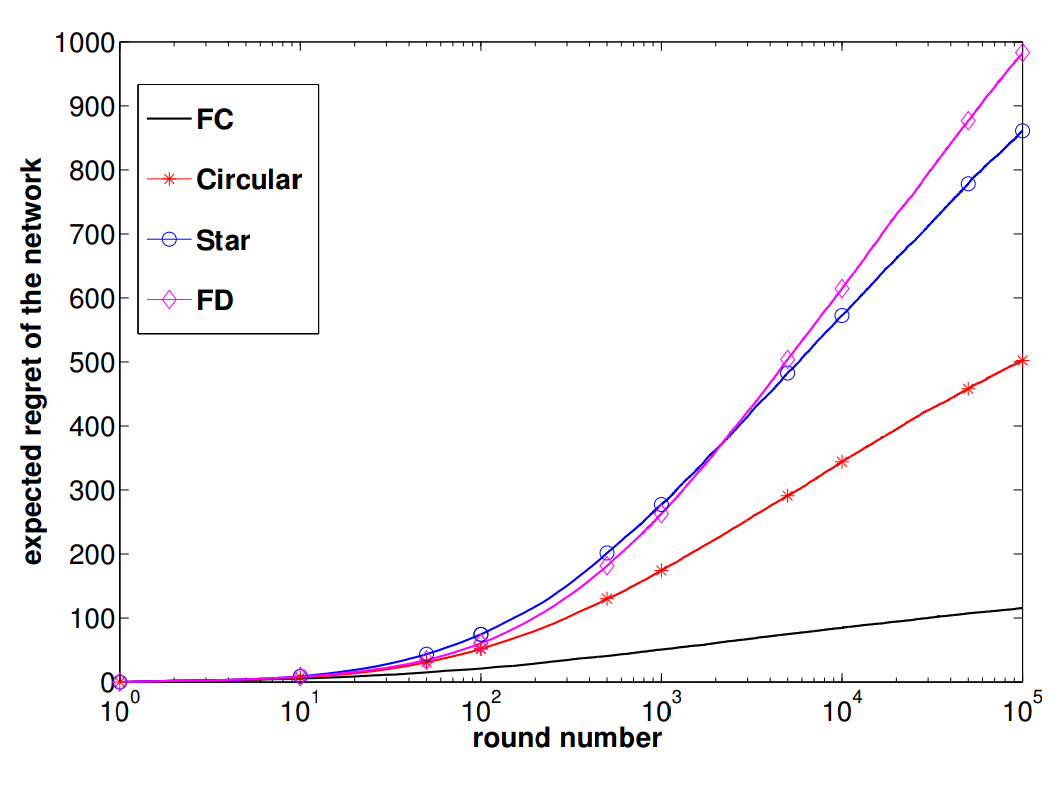
\includegraphics[width=0.49\linewidth]{fig1_1.png}
  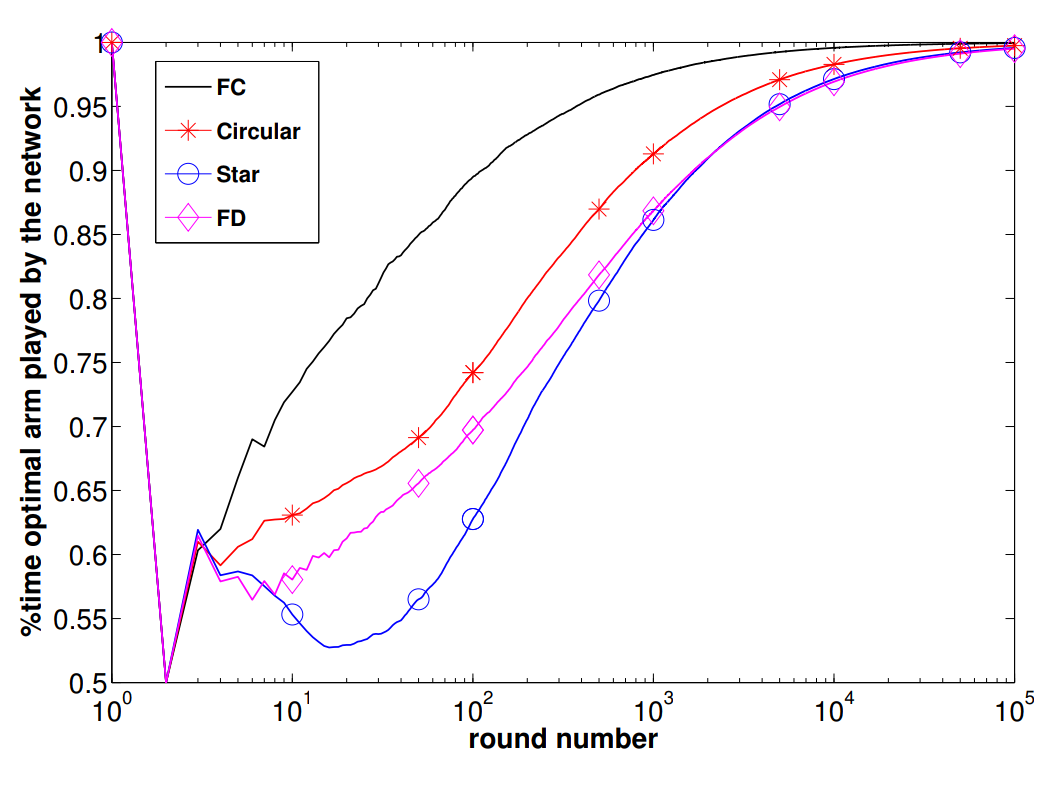
\includegraphics[width=0.49\linewidth]{fig1_2.png}
  \caption{Results for experiment 1 from \cite{DBLP:journals/corr/KollaJG16} (100 sample paths).}
\end{figure}

\begin{figure}[H]
  \centering
  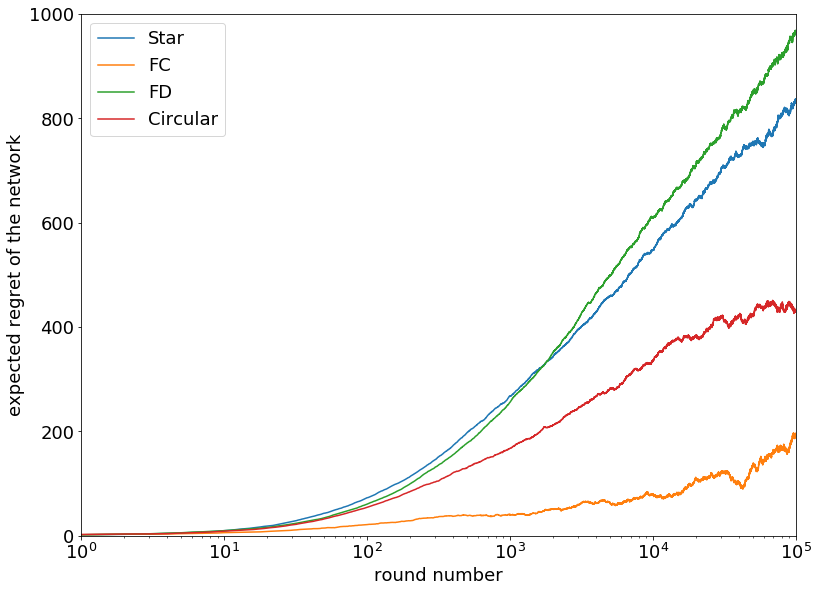
\includegraphics[height=5cm]{fig1_1_ours.png}
  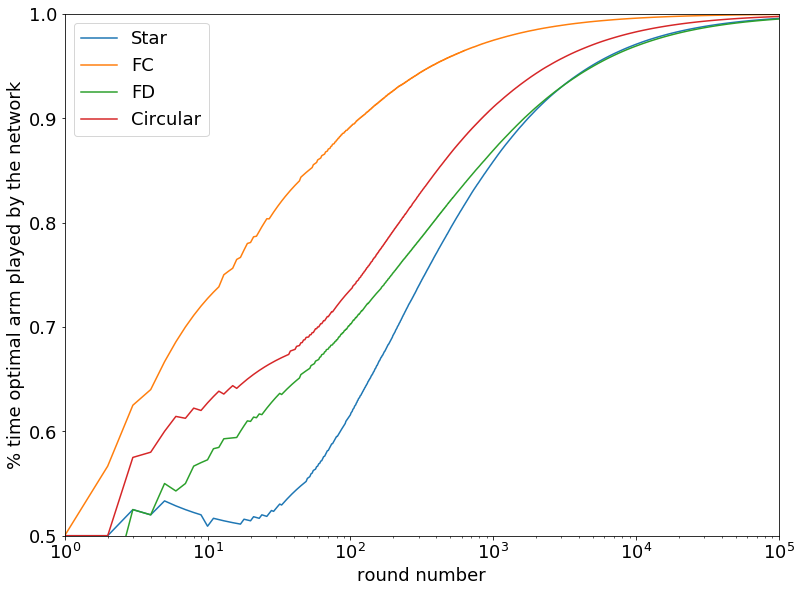
\includegraphics[height=5cm]{fig1_2_ours.png}
  \caption{Our results for experiment 1 (1000 sample paths).}
\end{figure}

We observe that we obtain exactly the same results as in \cite{DBLP:journals/corr/KollaJG16}, except for the expected regret of the network at rounds $ > 10000$. We get a noisier regret, even though we increased the number of simulations up to 1000 sample paths. We think that the authors of \cite{DBLP:journals/corr/KollaJG16} decided to smooth their curves.

\subsubsection{Experiment 2}

Performance comparison of UCB-Network policy on various 20 node networks: 10 arms, Bernoulli rewards with means $0.1, 0.2, \dots, 1$.

\begin{figure}[H]
  \centering
  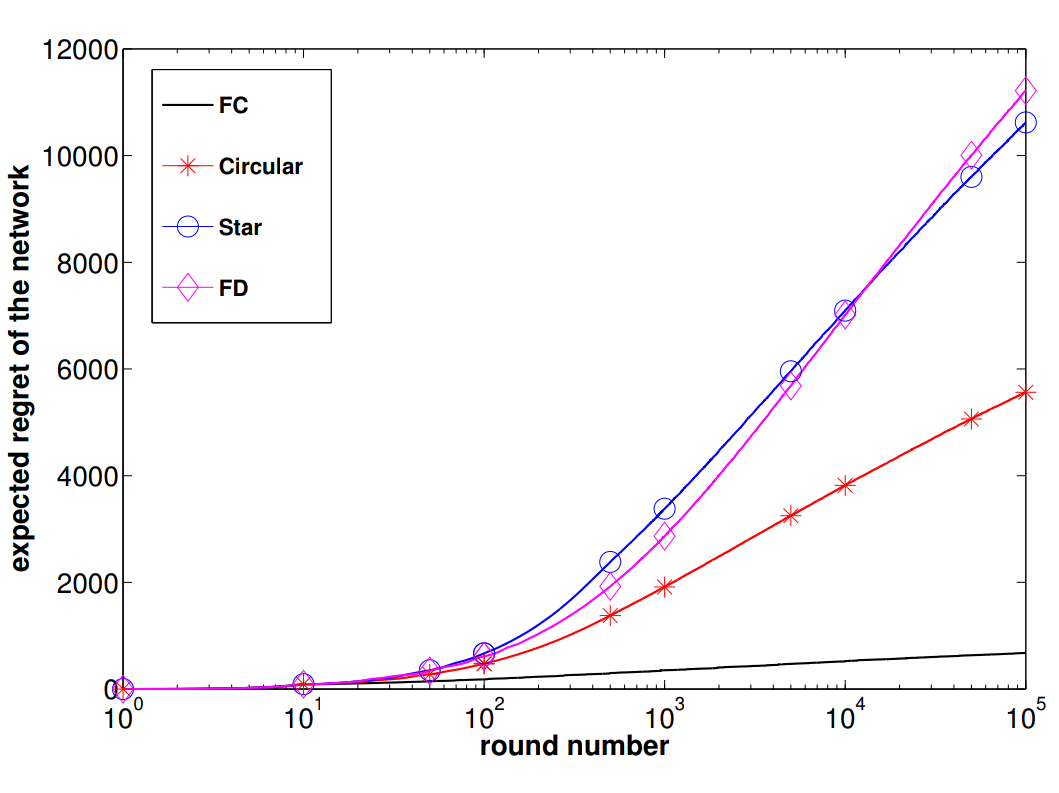
\includegraphics[width=0.49\linewidth]{fig2_1.png}
  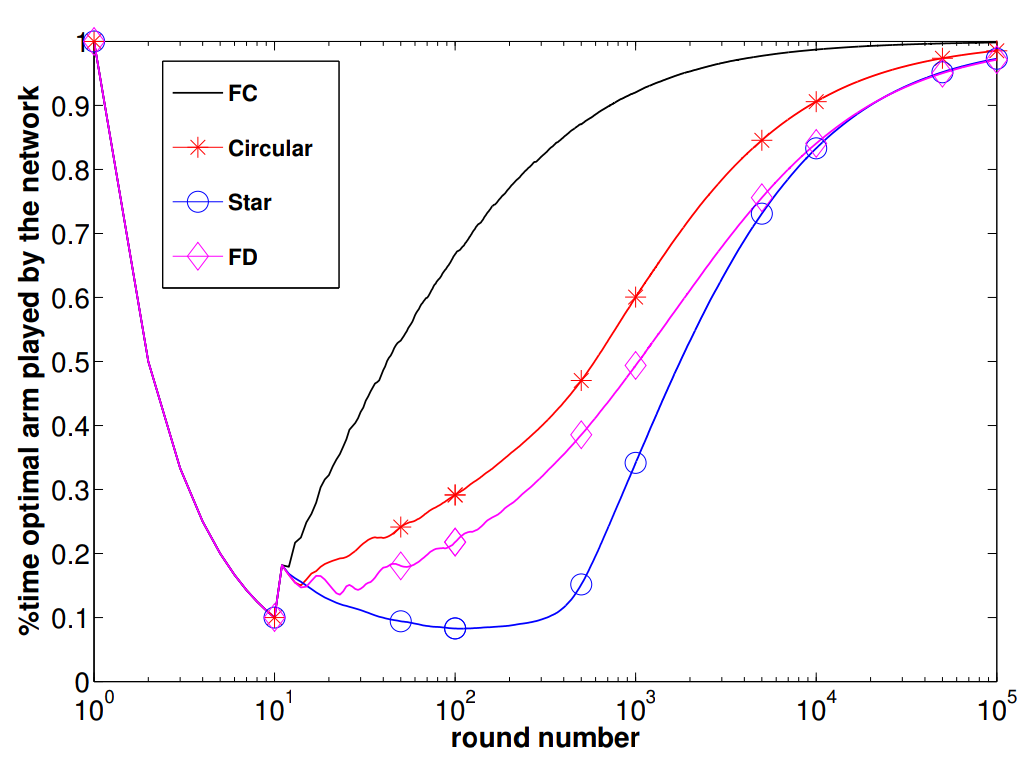
\includegraphics[width=0.49\linewidth]{fig2_2.png}
  \caption{Results for experiment 2 from \cite{DBLP:journals/corr/KollaJG16} (100 sample paths).}
\end{figure}

\begin{figure}[H]
  \centering
  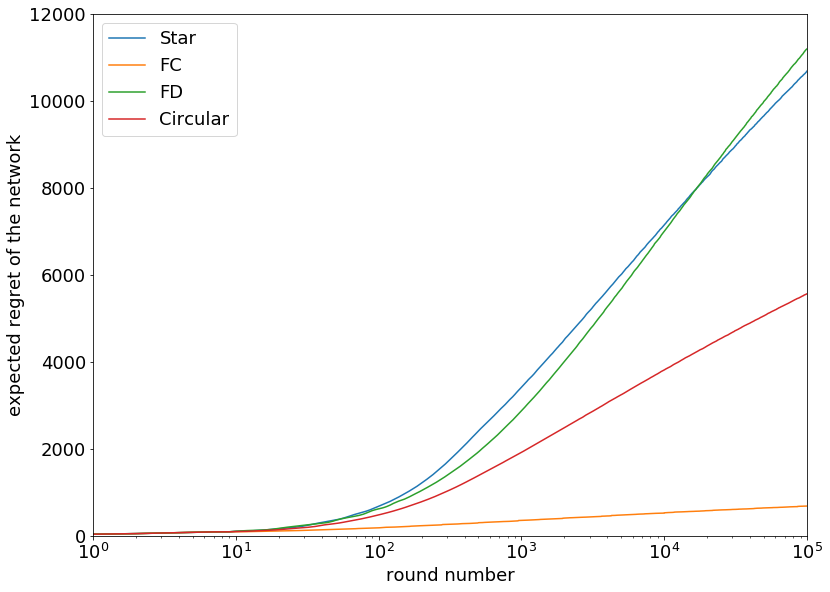
\includegraphics[width=0.49\linewidth]{fig2_1_ours.png}
  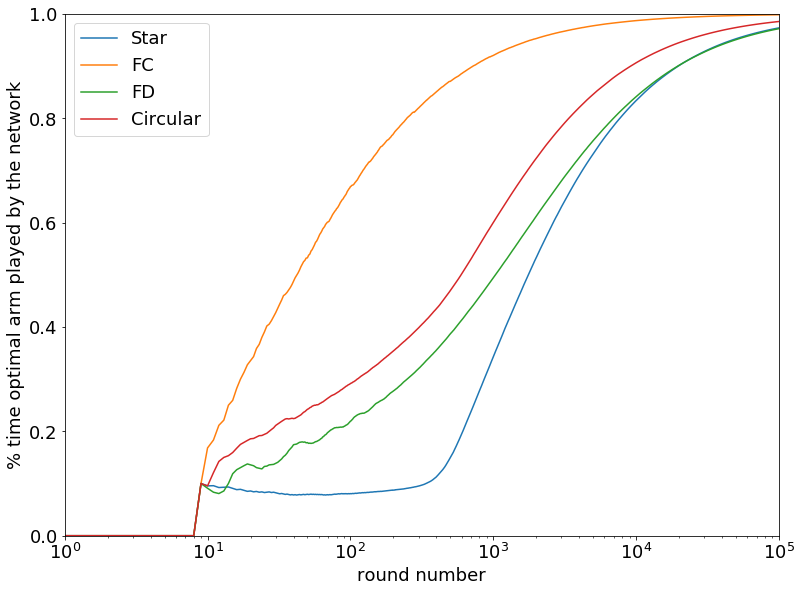
\includegraphics[width=0.49\linewidth]{fig2_2_ours.png}
  \caption{Our results for experiment 2 (1000 sample paths).}
\end{figure}

Here, we obtain the exact same results as in \cite{DBLP:journals/corr/KollaJG16}.

\subsubsection{Experiment 3}

Performance comparison of UCB-Network and FYL policies on various star networks: 2 arms, Bernoulli rewards with means $0.5$ and $0.7$.

\begin{figure}[H]
  \centering
  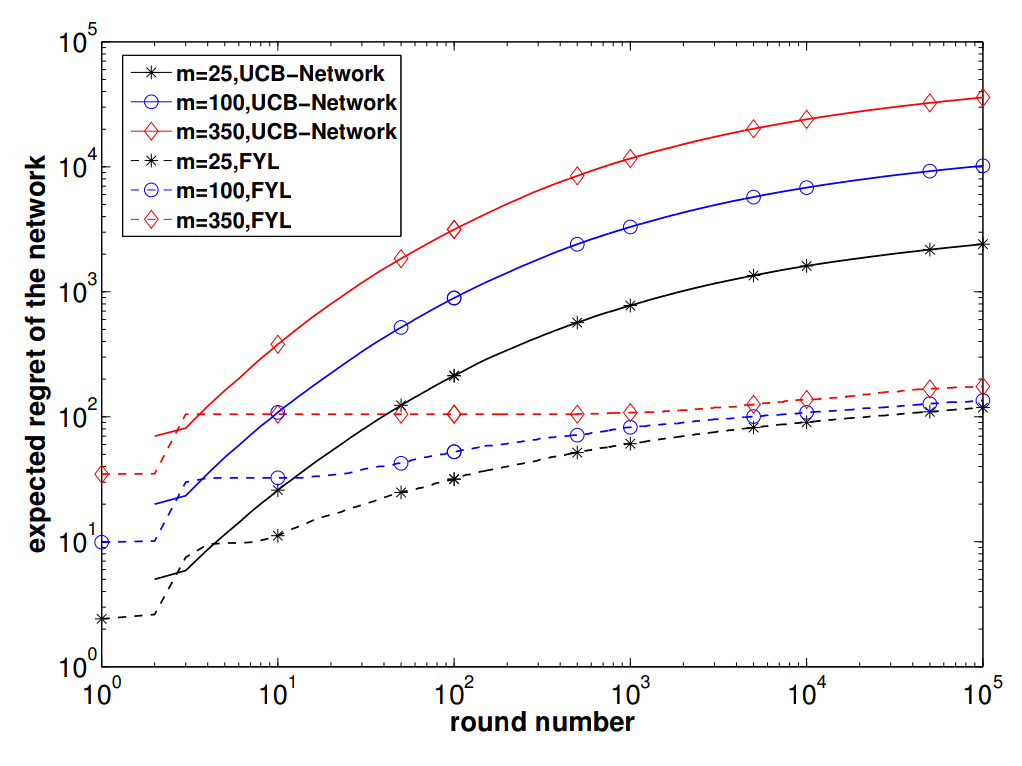
\includegraphics[width=0.49\linewidth]{fig3_1.png}
  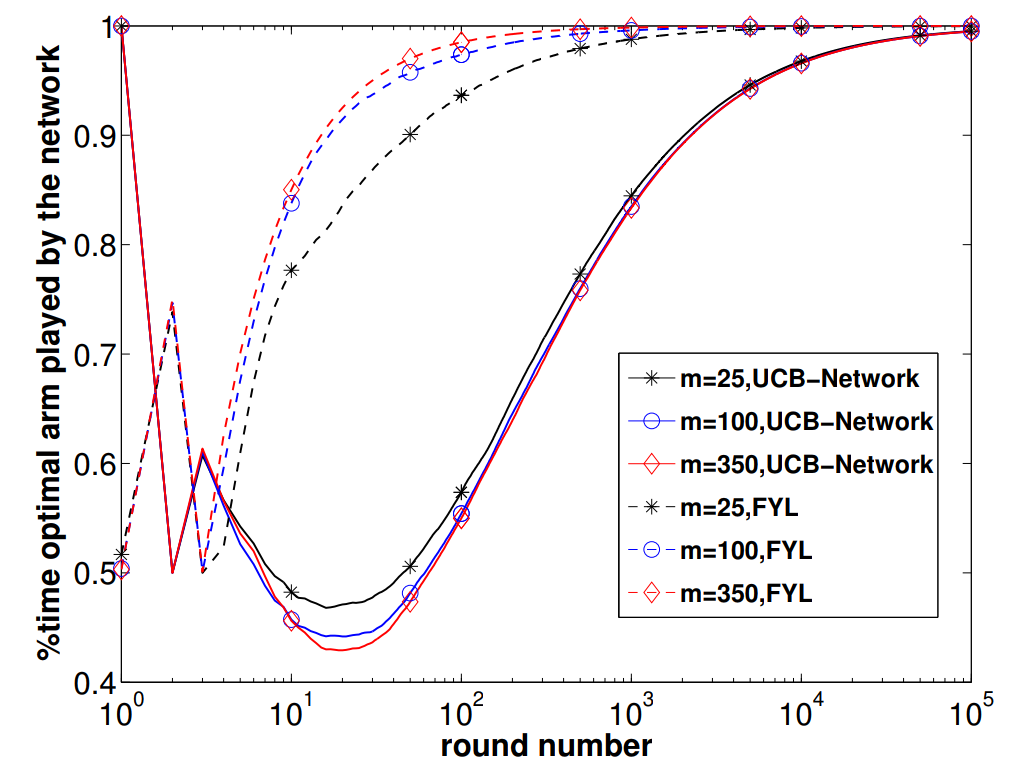
\includegraphics[width=0.49\linewidth]{fig3_2.png}
  \caption{Results for experiment 3 from \cite{DBLP:journals/corr/KollaJG16} (100 sample paths).}
\end{figure}

\begin{figure}[H]
  \centering
  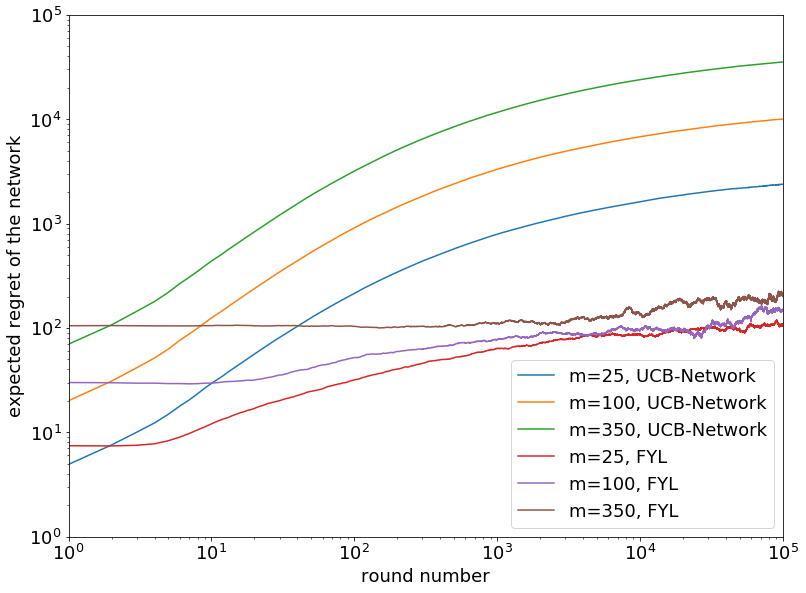
\includegraphics[width=0.49\linewidth]{fig3_1_ours.png}
  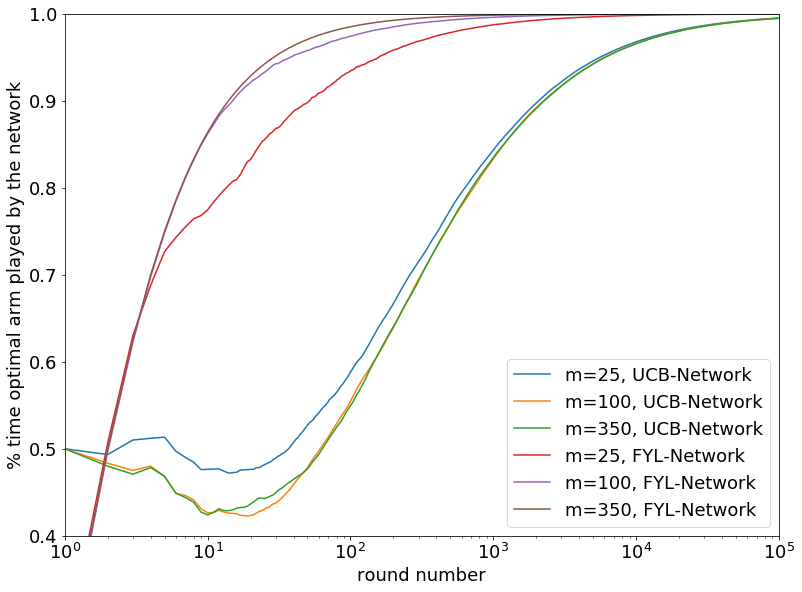
\includegraphics[width=0.49\linewidth]{fig3_2_ours.png}
  \caption{Our results for experiment 3 (1000 sample paths).}
\end{figure}

Same observation here as for experiment 1: we notice that we obtain exactly the same results as in \cite{DBLP:journals/corr/KollaJG16}, except for the expected regret of the network at rounds $ > 10000$. We get a noisier regret, even though we increased the number of simulations up to 1000 sample paths. We think that the authors of \cite{DBLP:journals/corr/KollaJG16} decided to smooth their curves.

\subsection{Evaluating Follow Best Informed (FBI) policy}
\label{FBI}

\subsubsection{Comparison between star network and multiple stars network}

Finally, we provide experimental results to demonstrate the efficiency our Follow Best Informed (FBI) policy.

We show that it provides similar results as FYL for star networks, and improves the performance for general networks (here, multiple fully connected stars network, see Figure \ref{fcstars}).

\begin{figure}[H]
  \centering
  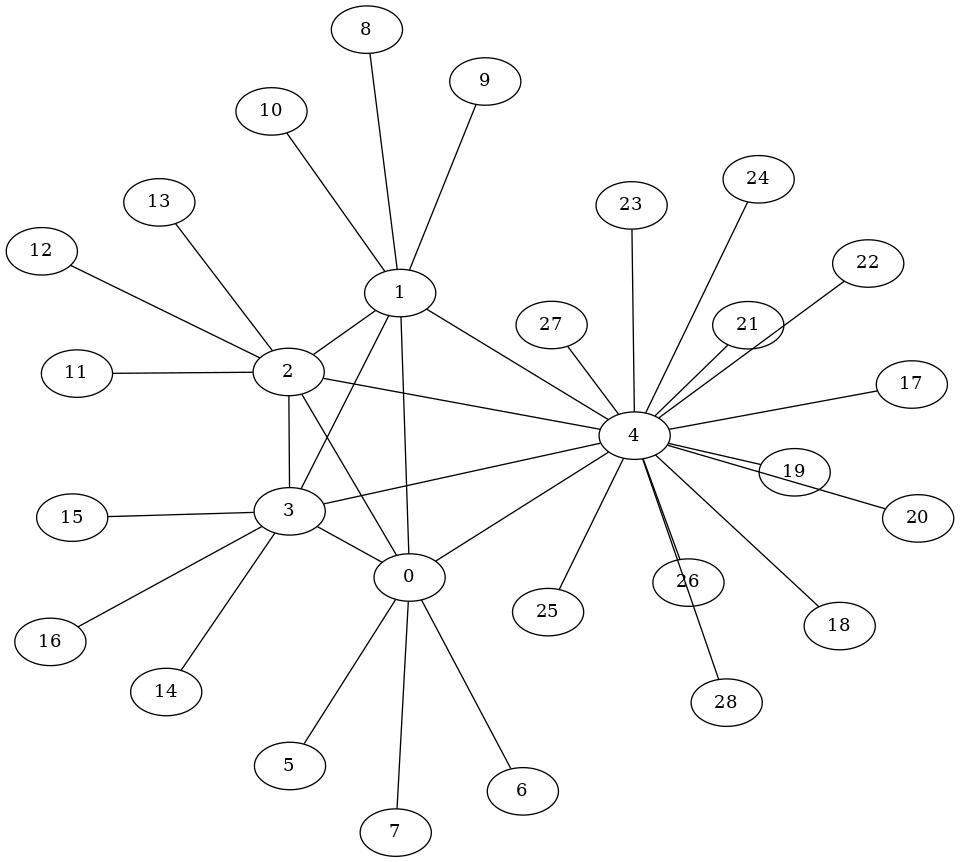
\includegraphics[width=0.6\linewidth]{fcstars.jpg}
  \caption{A 29-nodes 5-FC-stars network. It can be seen as a star network where the central hub got split into several sub-hubs.}
  \label{fcstars}
\end{figure}

\begin{figure}[H]
  \centering
  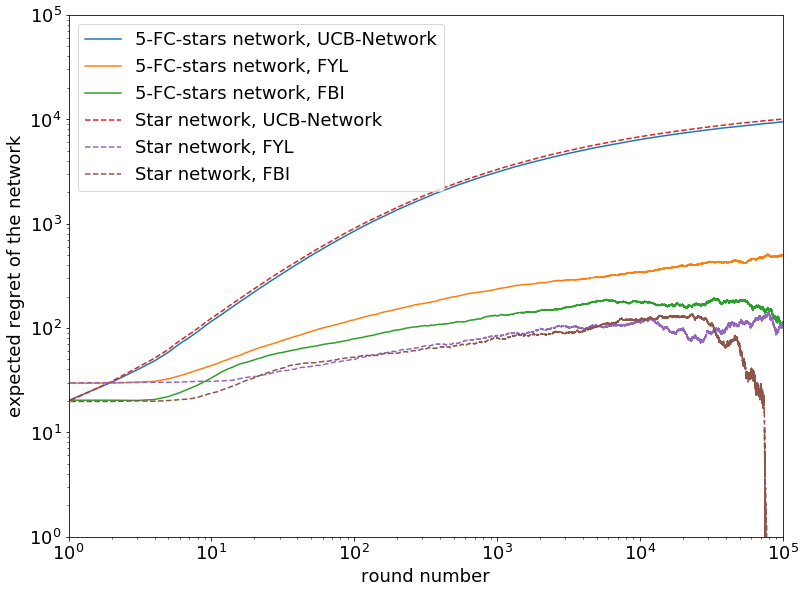
\includegraphics[width=0.49\linewidth]{fig4_1.png}
  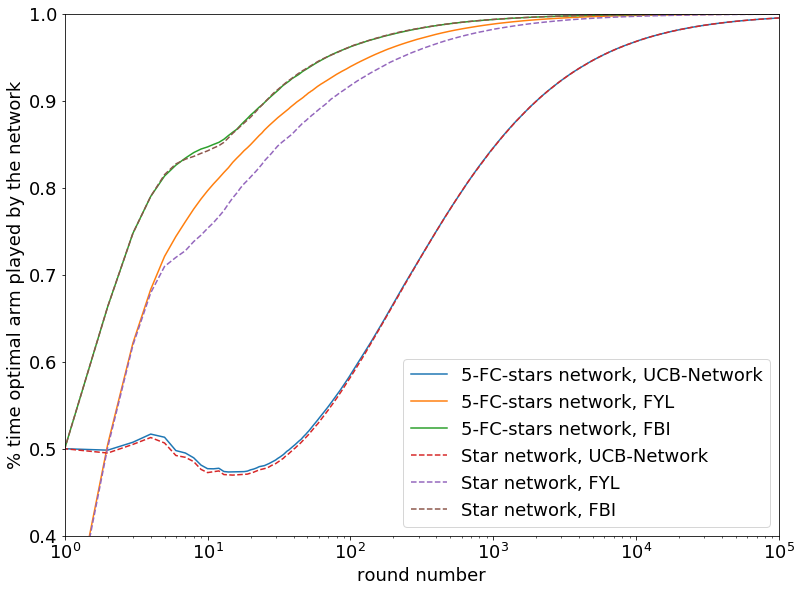
\includegraphics[width=0.49\linewidth]{fig4_2.png}
  \caption{Performance comparison of UCB-Network, FYL, and FBI policies on a 100-nodes star network and on the 100-nodes 5-FC-stars network: 2 arms, Bernoulli rewards with means $0.5$ and $0.7$ (1000 sample paths).}
\end{figure}

As expected, FYL and FBI policies perform about the same on star and multiple stars networks. But the great improvement of FBI over FYL lies in its ability to naturally adapt to the graph structure. It greatly decreases expected regret for the multiple stars network, compared to FYL.

\subsubsection{FYL can be really expensive on general graphs}

This gap is even larger on more pathological graph structure. Here, we compare FYL and FBI on this kind of graphs:

\begin{figure}[H]
  \centering
  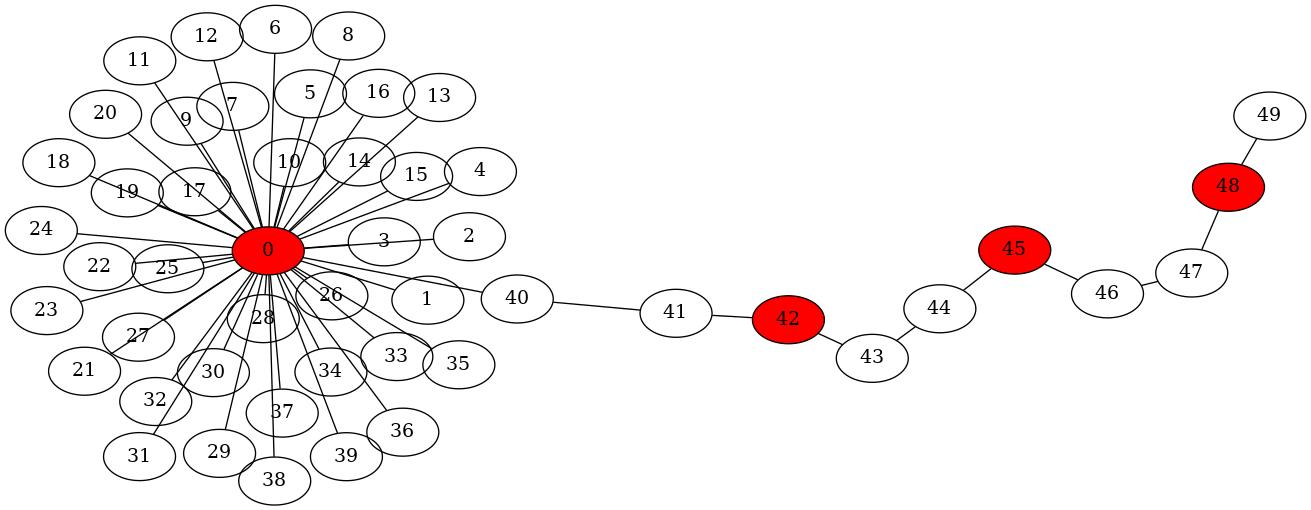
\includegraphics[width=0.6\linewidth]{star-chain.jpg}
  \caption{A pathological graph structure. The minimum dominating set is indicated in red.}
\end{figure}

\begin{figure}[H]
  \centering
  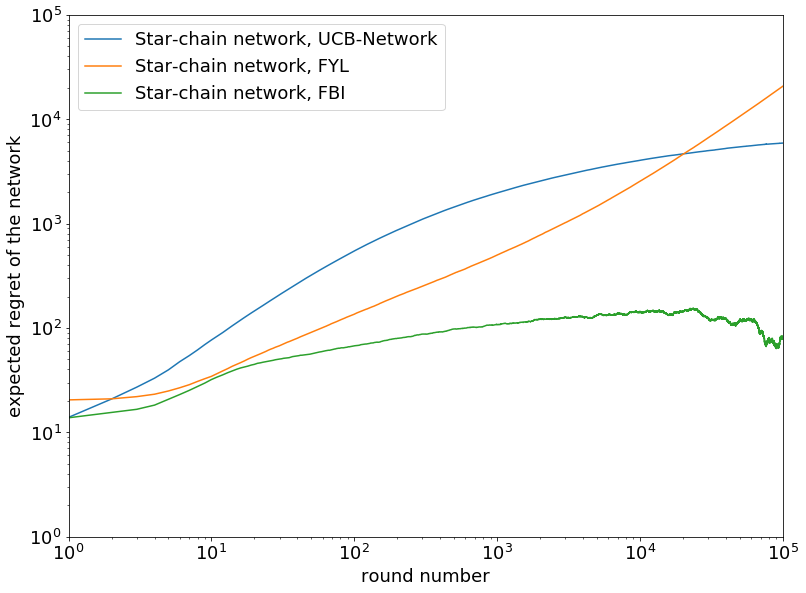
\includegraphics[width=0.49\linewidth]{fig5_1.png}
  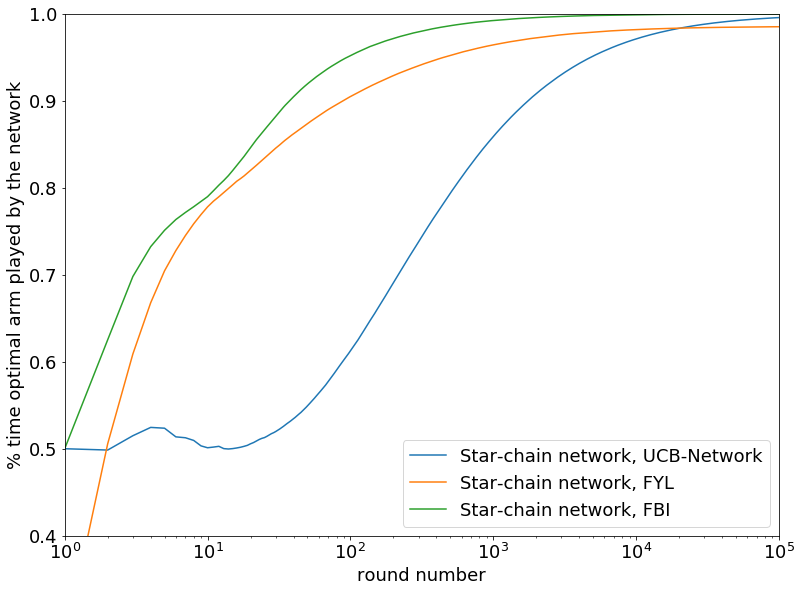
\includegraphics[width=0.49\linewidth]{fig5_2.png}
  \caption{Performance comparison of FYL and FBI policies on the pathological graph structure (star graph with 70 nodes, among which a 20-nodes long chain): 2 arms, Bernoulli rewards with means $0.5$ and $0.7$ (1000 sample paths).}
\end{figure}

One issue of FYL is that it doesn't really take into account the full structure of the graph, and can only benefit from star structures. The more general the graph, the worst the policy. This comes from the fact that FYL policy relies on the dominating set (see upper bound of Theorem 6 from \cite{DBLP:journals/corr/KollaJG16}). In our example, the dominating set doesn't allow children nodes to collect samples efficiently, so FBI performs much better than FYL.

\section{Conclusion}

% FIXME Conclusion

{\small
\bibliographystyle{unsrt}
\bibliography{biblio}
}

\end{document}
